\documentclass{beamer}

\usepackage{braket}


% Choose a theme
\usetheme{default}
\setbeamertemplate{footline}[frame number]

\setcounter{MaxMatrixCols}{15}

\title{[[15, 7, 3]] Testing}

\begin{document}

\maketitle

\begin{frame}{Motivation}
    I looked for error correcting codes with more physical qubits with multiple logical qubits and distance at least 3 for basic error correction. I found the [[15, 7, 3]] quantum Hamming code to satisfy all these requirements, as well as having a simple stabilizer structure for me to understand. 
\end{frame}

\begin{frame}{Stabilizers}
    The stabilizers mirror the parity check stabilizers of the classical Hamming, in both X and Z
    \footnotesize

    \[
    S = 
    \begin{pmatrix}
    S_1 \\ S_2 \\ S_3 \\ S_4 \\ S_5 \\ S_6 \\ S_7 \\ S_8
    \end{pmatrix}
    =
    \begin{pmatrix}
        X & X & X & X & X & X & X & X & I & I & I & I & I & I & I \\
        X & X & X & X & I & I & I & I & X & X & X & X & I & I & I \\
        X & X & I & I & X & X & I & I & X & X & I & I & X & X & I \\
        X & I & X & I & X & I & X & I & X & I & X & I & X & I & X \\
        Z & Z & Z & Z & I & I & I & I & I & I & I & I & I & I & I \\
        Z & Z & Z & Z & I & I & I & I & Z & Z & Z & Z & I & I & I \\
        Z & Z & I & I & Z & Z & I & I & Z & Z & I & I & Z & Z & I \\
        Z & I & Z & I & Z & I & Z & I & Z & I & Z & I & Z & I & Z \\
    \end{pmatrix}
    \]
    \normalsize
    Here I've got them backwards from the usual convention, this is so that the syndrome identifies the error qubit indexed from the right, using the binary concatenation of the 4 stabilizers of each type. (ex. $S_1S_2S_3S_4 = 0001$ corresponds to the first qubit from the right)
\end{frame}

\begin{frame}{Simulation - General Structure}
    Typical circuit structure for stim simulation:
    \begin{enumerate}
        \item Initialize circuit with all physical qubits in $\ket{0}$, there are 15 physical qubits and 8 ancilla qubits.
        \item Warmup round - same noise round as described in next point, measure the 8 stabilizers as the initial state. 
        \item Noise round - perform ancilla/data coupling in time windows to represent optimal scheduling. For simplicity, complete Z type stabilizers first and then X type stabilizers to ensure no cross interference. This should give 8 time windows per stabilizer type with 4 ancilla couplings per time window. These stabilizers are measured again and their xor with the previous round gives the syndrome.
        \item Logical readout - for now I am just measuring all 15 physical qubits for Z type logical operator. Working to redesign this to measure more logical operators to get better idea of error per logical qubit.
    \end{enumerate}
\end{frame}

\begin{frame}{Simulation - Verification}
    To double check my implementation, I created a modified version to inject errors onto physical and/or ancilla qubits in otherwise zero noise. Here is the behavior I observe:
    \begin{itemize}
        \item A single error on a physical qubit will be detected properly by syndrome measurement (good) as long as there is no error on the corresponding ancilla.
        \item Multiple errors of the same type on physical qubits is detected as the sum of the bitstrings on the ancilla qubits, so this fails to detect the error. One x error and one z error can be detected properly by the syndrome measurements (expected).
        \item Ancilla errors are detrimental and will lead to logical error.
    \end{itemize}
    Overall, this is expected behavior, and I continue with the simulation.
\end{frame}

\begin{frame}[fragile]{Simulation - Scheduling}
    Simple schedule of the noise round for each stabilizer type, the number is the time window during which that qubit is coupled to ancilla. 
    \begin{verbatim}
        12345678-------
        2345----6781---
        34--67--12--58-
        4-5-1-2-3-6-7-8
    \end{verbatim}
    Due to the weight 8 stabilizers, this requires 8 time windows for each stabilizer type, 16 in total, 4 couplings per time window. In the entire noise round, this is 64 gates.
\end{frame}

\begin{frame}{Simulation - Decoding}
    In my first test, I used Pymatching for decoding, but the results looked higher than expected, so to double check I manually decoded based on the measurements in each round:
    \begin{enumerate}
        \item Calculate detector for each round (ex. round 1 $\oplus$ warmup) 
        \item Flip measured bit at indicated index. Since I am measuring the logical oeprator in Z, I am only looking at the Z type syndrome (first 4 bits).
        \item Compare final bitstring to most similar codeword to see if it gives the correct logical readout and if it is outside the codespace. 
    \end{enumerate}
    Since I am manually decoding, I can also keep track of successful corrections and harmful corrections and how they affect logical error rate. I determine if a logical readout is correct by checking that it is equal to the expected value and that it is preserved in the codespace, ie it matches a codeword for this logical operator.
\end{frame}

\begin{frame}{Simulation - Decoding (checking codewords)}
    Running the circuit with no noise, I can sample all of codewords for the logical operator of all 15 physical qubits by observing that the final state after 1 round is uniformly distributed over 16 codewords.Here is what I find:
    \tiny
    \begin{align*}
        \ket{0}_Z = \frac{1}{\sqrt{16}}(&\ket{000000000000000}+\ket{000011111111000}+\ket{001100111100110}+\ket{001111000011110}\\+&\ket{010101011010101}+\ket{010110100101101}+\ket{011001100110011}+\ket{011010011001011}\\+&\ket{100101101001011}+\ket{100110010110011}+\ket{101001010101101}+\ket{101010101010101}\\+&\ket{110000110011110}+\ket{110011001100110}+\ket{111100001111000}+\ket{111111110000000})
        \\\ket{1}_Z = \frac{1}{\sqrt{16}}(&\ket{000000001111111}+\ket{000011110000111}+\ket{001100110011001}+\ket{001111001100001}\\+&\ket{010101010101010}+\ket{010110101010010}+\ket{011001101001100}+\ket{011010010110100}\\+&\ket{100101100110100}+\ket{100110011001100}+\ket{101001011010010}+\ket{101010100101010}\\+&\ket{110000111100001}+\ket{110011000011001}+\ket{111100000000111}+\ket{111111111111111})
    \end{align*}
    \normalsize
\end{frame}

\begin{frame}{Simulation - Parameter Sweep}
    Chose a small set for now:
    \begin{itemize}
        \item Num noise rounds - 1, 2, 3, 4, 5, 10, 20, 30, 40, 50
        \item Error rate - 1e-4, 2e-4, 5e-4, 1e-3, 2e-3, 5e-3
    \end{itemize}
    10000 shots per parameter pair, 60 total runs. Keeping track of:
    \begin{itemize}
        \item Logical error rate (LER) - proportion where logical readout is incorrect. We expect 0 since initialized in all $\ket{0}$.
        \item Outside codespace - proportion where final state is outside the codespace, found by comparing to most similar codeword.
        \item Detector fires - proportion where a detectors fire, rough indicator of how many physical errors occur.
        \item Successful corrections - proportion where error correction in decoding gives correct logical readout.
        \item Harmful corrections - proportion where error correction in decoding gives incorrect logical readout when it was correct before.
    \end{itemize}
\end{frame}

\begin{frame}{Simulation - Noise Model}
    For now, I only introduce noise on single qubit gates and CNOTs, in the form of uniform depolarizing noise. I have no error on the measurement operations right now, the idea is to isolate the effect of the stabilizer circuit on the overall noise and logical error. Also, since I'm measuring all 15 physical qubits at the end of the experiment, I don't want to introduce possibly significant error on the logical readout just from measurement noise. I think I will be able to reincorporate this as I shift to measuring more logical operators, which can be as low-weight as 3 physical qubits. Again, right now I am measuring all 15 physical qubits to see the entire behavior.
\end{frame}

\begin{frame}{Gauge}
    Taking the idea of "promoting" a logical operator to a stabilizer, I took the logical operator $\bar X = XXXXIIIIIIIIIII$ and added it as a gauge operator in the stabilizer group. I chose this logical operator because it overlaps with $S_1$ and $S_2$ and I can "decompose" these by measuring the modulo, giving:
    \begin{align*}
        G_1 &= XXXXIIIIIIIIIII \\
        G_2 &= IIIIXXXXIIIIIII \\
        G_3 &= IIIIIIIIXXXXIII
    \end{align*}
    Then we can recover the stabilizers by
    \begin{align*}
        S_1 &= G_1G_2 \\
        S_2 &= G_1G_3
    \end{align*}
    To be sure this is a valid logical operator, some choices for complimentary $\bar Z$ are $IIIZZIIIZIIIIII$ and $IIZIIZIIZIIIIII$, for example. These anticommute with $\bar X$ but commute with all stabilizers.
\end{frame}

\begin{frame}{Gauge}
    Then the full gauge group is:
    \footnotesize
    \[G = 
    \begin{pmatrix}
    G_1 \\ G_2 \\ G_3 \\ G_4 \\ G_5 \\ G_6 \\ G_7 \\ G_8 \\ G_9 \\ G_{10} \\ G_{11} \\ G_{12} \\
    \end{pmatrix}
    =
    \begin{pmatrix}
    X & X & X & X & I & I & I & I & I & I & I & I & I & I & I \\
    I & I & I & I & X & X & X & X & I & I & I & I & I & I & I \\
    I & I & I & I & I & I & I & I & X & X & X & X & I & I & I \\
    X & I & I & I & X & I & I & I & X & I & I & I & X & I & I \\
    I & X & I & I & I & X & I & I & I & X & I & I & I & X & I \\
    I & I & X & I & I & I & X & I & I & I & X & I & I & I & X \\
    Z & Z & Z & Z & I & I & I & I & I & I & I & I & I & I & I \\
    I & I & I & I & Z & Z & Z & Z & I & I & I & I & I & I & I \\
    I & I & I & I & I & I & I & I & Z & Z & Z & Z & I & I & I \\
    Z & I & I & I & Z & I & I & I & Z & I & I & I & Z & I & I \\
    I & Z & I & I & I & Z & I & I & I & Z & I & I & I & Z & I \\
    I & I & Z & I & I & I & Z & I & I & I & Z & I & I & I & Z \\
    \end{pmatrix}\]
    \normalsize
    And the stabilizers are recovered by:
    \begin{align*}
        S_1 &= G_1G_2 \quad S_3 = G_4G_5 \quad S_5 = G_7G_8 \quad S_7 = G_{10}G_{11} \\
        S_2 &= G_1G_3 \quad S_4 = G_4G_6 \quad S_6 = G_7G_9 \quad S_8 = G_{10}G_{12}
    \end{align*}
\end{frame}

\begin{frame}[fragile]{Gauge - Scheduling}
    \begin{verbatim}
        1234-----------
        ----1234-------
        --------1234---
        2---3---4---1--
        -3---4---1---2-
        --4---1---2---3
    \end{verbatim}
    By decomposing the stabilizers, we can now perform each stabilizer type coupling in 4 time windows coupling 6 physical qubits in each window, for a total of 24 gates for each stabilizer type, and 48 gates in total. Each stabilizer is now weight 4.
\end{frame}

\begin{frame}{Gauge - Verification, Decoding, Simulation}
    Decoding is done in a similar way as the original code, except the stabilizers are computed for each round before applying the XOR for the detector syndrome. \\
    \vspace{0.5cm}
    I used the same error injection method to verify the code works as expected. We see individual G gauge operators fluctuate each round, but the reconstructed stabilizers follow expected behavior.\\
    \vspace{0.5cm}
    I simulated with the same parameter sweep and noise model as the original code.
\end{frame}

\begin{frame}{Results - LER}
    \begin{figure}
        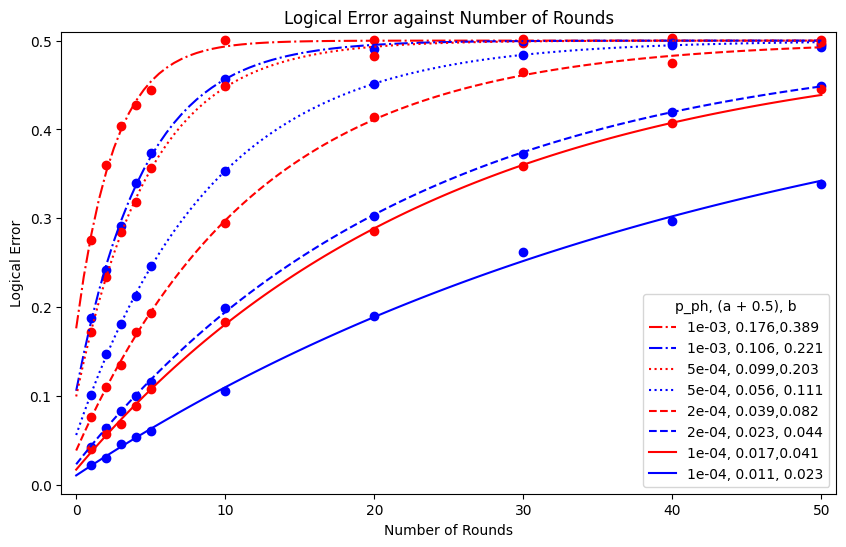
\includegraphics[width=\textwidth]{ler.png}
    \end{figure}
\end{frame}

\begin{frame}{Results - LER}
    LER comparison across different physical error rates and number of noise rounds. Red is the original code, blue is the gauge code. I have plotted the simulation datapoints up to $er = 1e-3$ so its not so clustered, and an exponential decay function which asymptotes to 0.5.
    \[LER(N) = a \exp(-bN) + 0.5\]
    Here $a$ is the amplitude, which is a negative number, so the value $(a+0.5)$ represents the y-intercept, or the error introduced by the warmup round, since no syndrome is measured. $b$ is the decay rate, follows a trend we expect. \\
    \vspace{0.5cm}
    This plot generally shows that the gauge code LER grows slower. But remember that this is LER for a single logical qubit, I will do more tests for per-logical qubit LER.
\end{frame}

\begin{frame}{Results - error correction power}
    \begin{figure}
        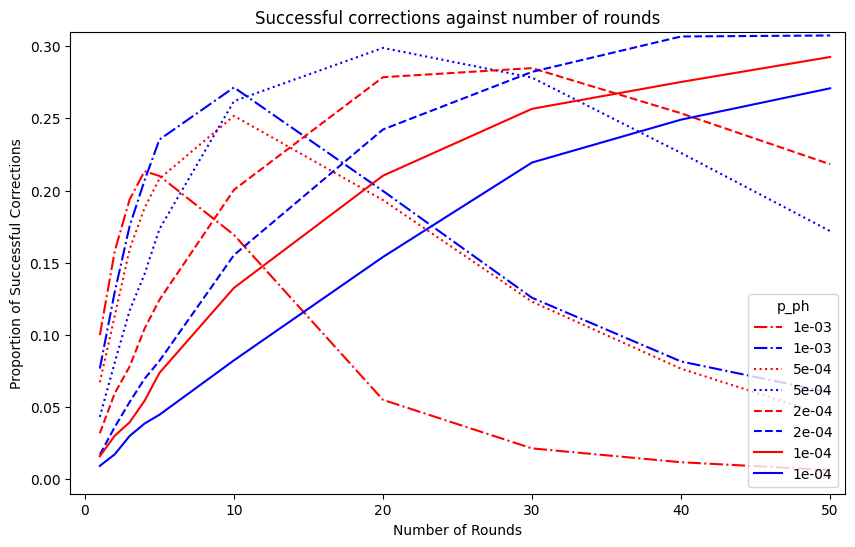
\includegraphics[width=\textwidth]{successful.png}
    \end{figure}
\end{frame}

\begin{frame}{Results - error correction power}
    \begin{figure}
        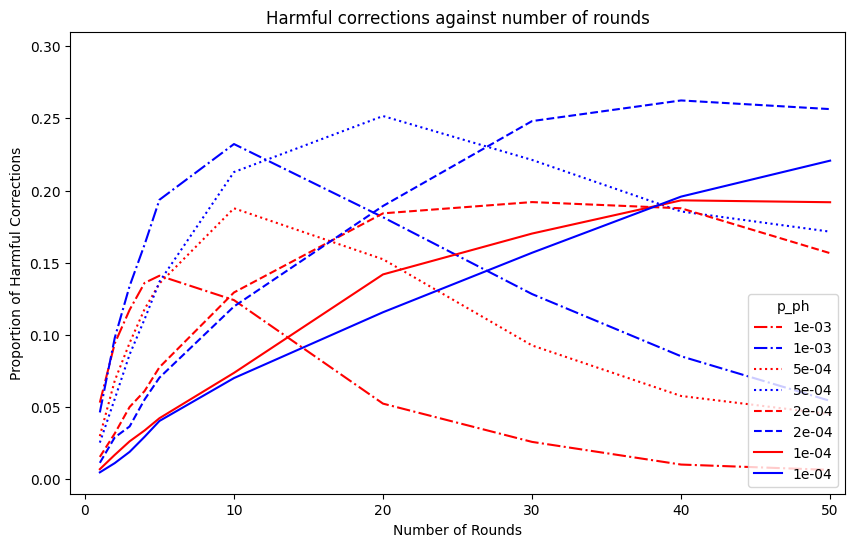
\includegraphics[width=\textwidth]{harmful.png}
    \end{figure}
\end{frame}

\begin{frame}{Results - error correction power}
    \begin{figure}
        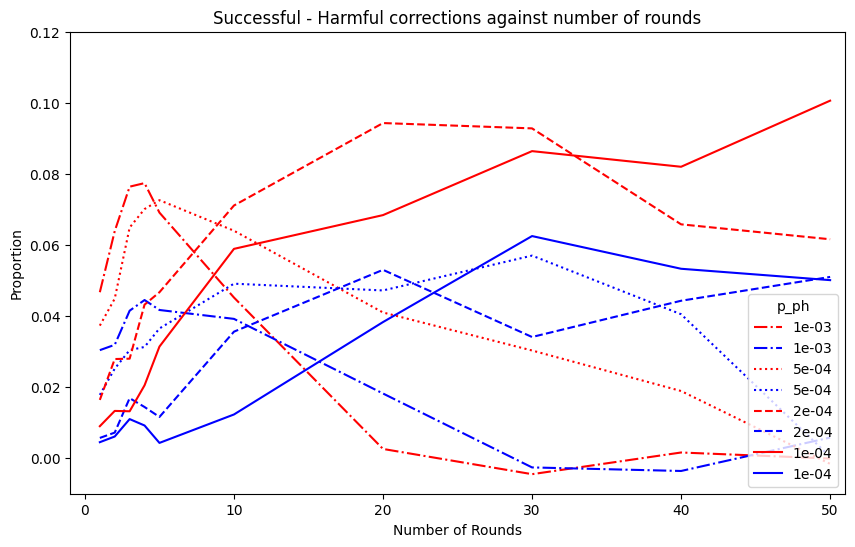
\includegraphics[width=\textwidth]{successharm.png}
    \end{figure}
\end{frame}

\begin{frame}{Results - error correction power}
    I call the code's ability to properly correct errors the "error correction power". This is also important to explain part of the LER.\\
    \vspace{0.5cm}
    The three plots compare successful corrections, harmful corrections, and the difference between the two. What I generally observe is that for both successful and harmful corrections, the gauge grows slower and peaks higher, the net effect of which is in generally slightly worse correction power in the gauge code. So it seems that the primary benefit of the gauge code is to just reduce the probability that errors happen in the first place.\\
    \vspace{0.5cm}
    I need to do some investigation to understand why both the successful and harmful corrections rise higher for the gauge code.
\end{frame}

\begin{frame}{Comments}
    So far it seems that we get expected behavior from the simulation. But I don't think this is yet gauging in the sense that we are after. We are not really changing the codespace, just changing the way that we measure the syndrome. \\
    \vspace{0.5cm}
    What I do benefit from this study so far is I am learning a lot about the behavior of this sort of decomposition of the code.
\end{frame}

\begin{frame}{Next Steps}
    \begin{itemize}
        \item In order to truly gauge fix the code, I need to enforce $G_i = +1$, though I am not sure how this might affect the codespace.
        \item Implement more diverse logical readout for all logical degrees of freedom, moving away from just "monitoring" the final state.
        \item Add back measurement noise.
        \item Investigate error correction power.
        \item Move to different codes, this [[15, 7, 3]] is not super practical, but I do want to develop an understanding surrounding this idea of overlapping stabilizers.
    \end{itemize}
\end{frame}

\end{document}